\chapter{Appendix B: Neuron Model Equations}\label{app:neuron_equations}
\graphicspath{{../Figures/93-AppendixB/}{figs/93-AppendixB/}}

Both neuron models integrate current, and a membrane leak draws voltage toward rest. A nonspiking synapse varies its conductance continuously with presynaptic voltage over its operating range. A spiking neuron signals when its voltage crosses a threshold, and the resulting spike changes synaptic conductance. The same wiring can therefore produce different muscle commands. This appendix gives the equations and calibration used to compare these mechanisms in AnimatLab and Gait2392. Appendix~\ref{app:simulation_verification}, Section~\ref{sec:spiking_methods}, gives the resulting rhythm and motion. Section~\ref{sec:app_knee_transient} describes the nonspiking circuit built in the graphical editor for the biological knee. The final section of this appendix maps the sensory connections tested separately in W2L.

\section{Spiking Neuron Model}

In the archived AnimatLab walker, the spiking neuron is a conductance-based leaky integrator with a firing threshold and accommodation,
\begin{equation}
    C_{m}\,\dot{V} \;=\; -\,g_{\text{leak}}\left(V - E_{\text{rest}}\right)
                      \;+\; I_{\text{syn}} \;+\; I_{\text{app}},
    \label{eq:app_membrane}
\end{equation}
where $V$ is the membrane potential, $C_{m}$ the membrane capacitance ($g_{\text{leak}} = C_{m}/\tau_{m}$ with membrane time constant $\tau_{m}$), $E_{\text{rest}}$ the resting potential, $I_{\text{syn}}$ the summed synaptic current, and $I_{\text{app}}$ any applied (tonic stimulation) current. A spike is emitted when $V$ exceeds the firing threshold, after which $V$ resets and an after-hyperpolarization (AHP) of amplitude $A_{\text{AHP}}$ with time constant $\tau_{\text{AHP}}$ is applied; the threshold itself accommodates with the firing history (relative accommodation $r_{\text{acc}}$, time constant $\tau_{\text{acc}}$). Optional calcium channels are defined but disabled in the archived AnimatLab model ($G_{\text{max,Ca}} = 0$).

The parameter values shared by the neurons in the walker model are given in Table~\ref{tab:app_neuron}.

\begin{table}[htbp]
\caption{Spiking neuron parameters in the AnimatLab bipedal walker model
(\nolinkurl{Biped_2xCPG_wSubs}). All neurons share these values except the motor
neuron threshold noted below.}
\label{tab:app_neuron}
\small\begin{tabularx}{\textwidth}{@{}>{\raggedright\arraybackslash}p{0.32\textwidth}lL@{}}
\toprule
\textbf{Parameter} & \textbf{Symbol} & \textbf{Value} \\
\midrule
Resting potential        & $E_{\text{rest}}$   & \qty{-60}{\mV} \\
Membrane time constant   & $\tau_{m}$          & \qty{5}{\ms}   \\
Initial firing threshold & $V_{\text{th}}$     & \qty{-55}{\mV} (motor neurons: \qty{-59}{\mV}) \\
Relative accommodation   & $r_{\text{acc}}$    & 0.3            \\
Accommodation time const & $\tau_{\text{acc}}$ & \qty{10}{\ms}  \\
AHP amplitude            & $A_{\text{AHP}}$    & \qty{1}{\mV}   \\
AHP time constant        & $\tau_{\text{AHP}}$ & \qty{3}{\ms}   \\
\bottomrule
\end{tabularx}
\end{table}

\section{Voltage-Dependent Chemical Synapses}

Pattern-formation and motoneuron-drive connections in the walker use voltage-dependent chemical synapses, whose conductance is a clipped linear ramp of the presynaptic potential,
\begin{equation}
    g_{\text{syn}}(V_{\text{pre}})
    \;=\; g_{\text{max}}\;
    \operatorname{clamp}\!\left(
        \frac{V_{\text{pre}} - V_{\text{th}}}{V_{\text{sat}} - V_{\text{th}}},
        \,0,\,1\right),
    \qquad
    I_{\text{syn}} = g_{\text{syn}}\left(E_{\text{syn}} - V_{\text{post}}\right),
    \label{eq:app_nonsyn}
\end{equation}
Here inward current is positive, consistently with Equation~\eqref{eq:app_membrane}; an excitatory reversal potential above the postsynaptic voltage therefore produces depolarization. The quantities $V_{\text{th}}$ and $V_{\text{sat}}$ are the synaptic threshold and saturation potentials and $E_{\text{syn}}$ the reversal potential. The walker model instantiates three nonspiking synapse types:

\begin{itemize}
    \item \textbf{Nicotinic ACh (excitatory drive):}
          $E_{\text{syn}} = \qty{-10}{\mV}$,
          $g_{\text{max}} = \qty{0.5}{\micro\siemens}$,
          $V_{\text{th}} \to V_{\text{sat}} = \qty{-65}{\mV} \to \qty{-20}{\mV}$.
    \item \textbf{Hyperpolarizing IPSP (inhibition):}
          $E_{\text{syn}} = \qty{-70}{\mV}$,
          $V_{\text{th}} \to V_{\text{sat}} = \qty{-55}{\mV} \to \qty{-40}{\mV}$.
    \item \textbf{Depolarizing IPSP:}
          $E_{\text{syn}} = \qty{-55}{\mV}$,
          $V_{\text{th}} \to V_{\text{sat}} = \qty{-60}{\mV} \to \qty{-40}{\mV}$.
\end{itemize}

Spiking chemical synapses and electrical synapses (rectifying coupling weight 0.1, non-rectifying 0.2) are also defined in the model and are available for the sensory afferent pathways of the MuJoCo/SNS implementation.

\section{Relation to the SNS-Toolbox Implementation}

SNS-Toolbox implements corresponding nonspiking and spiking conductance-based neurons and synapses \citep{nourse_sns_2023}. The AnimatLab parameters initialized a 410-neuron SNS-Toolbox network with per-leg rhythm-generator half-centers, phase-shifted pattern-formation groups, motoneuron pools for all 92 muscle-tendon actuators, and Ia, Ib, and II afferent populations. Its nonspiking equations have the forms of Equations~\eqref{eq:app_membrane} and~\eqref{eq:app_nonsyn}, with spiking threshold and accommodation removed. Afferent resting-tone offsets are zero, so Ia and Ib encode activity without a tonic offset.

Under tonic drive, the rhythm generator alternated between the legs. Applying a constant current $I_{\text{app}}$ to a motor neuron (MN), a pattern-formation neuron (PF), or a rhythm-generator neuron (RG) probes different stages of transmission. Section~\ref{sec:spiking_methods} gives the response of each tested implementation.

\section{Spiking-Mirror Implementation, Calibration, and Verification}\label{app:spiking_details}

To test the effect of changing the signaling mechanism, the spiking network retained the directed connections of its nonspiking counterpart. The conversion and calibration are implemented in \nolinkurl{Code/MuJoCo_SNS/spinal/build_network_spiking.py} and \nolinkurl{calibrate_spiking.py}. Their results are archived under \nolinkurl{Code/MuJoCo_SNS/spinal/reports_spiking_20261002/}. The corresponding Simulink blocks and tests are in \nolinkurl{Code/Matlab/SNS_Simscape/sns_build_spiking.m} and \nolinkurl{sns_units_test_spiking.m}.

\subsection{Adapting Integrate-and-Fire Cells and Hybrid Synapses}

Between spikes, every spiking cell of the MuJoCo mirror obeys the membrane equation
\begin{equation}
    C_{m}\,\dot{V} \;=\; -\,g_{m}\left(V - V_{\text{rest}}\right)
        \;+\; I_{\text{syn}} \;+\; I_{\text{bias}},
    \label{eq:app_lif}
\end{equation}
A spike occurs at threshold $\theta$, after which $V$ resets to $V_{\text{reset}}$ and $\theta$ increases by $\Delta\theta$. Between spikes, $\theta$ decays toward its initial value with time constant $\tau_{\theta}$, bounded by the adaptation floor. Tonic bias $I_{\text{bias}}$ places the equilibrium below threshold. Table~\ref{tab:app_spk_cells} gives the values used by SNS-Toolbox's \texttt{SpikingNeuron}; this archived implementation uses $g_m=\qty{1}{\micro\siemens}$ throughout to retain consistency with its specified current units.

The rhythm-generator adaptation time constant is inherited from the analog persistent-sodium inactivation value, \qty{0.35}{\second} at the rhythm test's operating point. In the contact-driven analog cores, that slowly inactivating inward current terminates bursts. Its inactivation time constant is fixed in the tested implementations because the voltage-dependent form quenched termination and left the network latched.

\begin{table}[htbp]
\caption{Spiking cell parameters of the MuJoCo mirror (real millivolts; \nolinkurl{build_network_spiking.py}, \texttt{SPIKE} table, with the rhythm-generator increment superseded by the calibration of record). All cells rest at \qty{-70}{\mV} with membrane conductance \qty{1}{\micro\siemens} and the tonic bias of Table~\ref{tab:app_spk_cal}.}
\label{tab:app_spk_cells}
\small\begin{tabularx}{\textwidth}{@{}>{\raggedright\arraybackslash}p{0.28\textwidth}LLLL@{}}
\toprule
\textbf{Cell class} & $\boldsymbol{\theta}$ (\unit{\milli\volt}) & $\boldsymbol{V_{\text{reset}}}$ (\unit{\milli\volt}) & $\boldsymbol{\Delta\theta}$ (\unit{\milli\volt}/spike) & $\boldsymbol{\tau_{\theta}}$ (\unit{\second}) \\
\midrule
Rhythm generator E/F & $-50$ & $-60$ & 4.0 (calibrated) & 0.35 (analog value) \\
Pattern-formation     & $-50$ & $-60$ & 0.3 & 0.15 \\
Interneurons, commissurals & $-50$ & $-60$ & --- & --- \\
Afferent encoders     & $-52$ & $-58$ & --- & --- \\
Renshaw               & $-52.5$ & $-58$ & --- & --- \\
\bottomrule
\end{tabularx}
\end{table}

Spiking chemical synapses, in both the toolbox class used in the MuJoCo mirror and the Simulink \texttt{SpikingSynapse} block, carry a conductance that decays between events and jumps by a fixed increment per presynaptic spike, saturating at its maximum,
\begin{equation}
    \dot{g} \;=\; -\,g/\tau_{\text{syn}} \;\;\text{between spikes}, 
    \qquad g \leftarrow \min\!\left(g_{\max},\, g + g_{\text{inc}}\right) \;\;\text{per spike},
    \label{eq:app_spk_syn}
\end{equation}
with $I_{\text{syn}} = g\,(E_{\text{syn}} - V_{\text{post}})$ as for the voltage-dependent synapse of Equation~(\ref{eq:app_nonsyn}). The Simulink \texttt{HybridSpikingSynapse} implements the same dynamics with the spike detected from the presynaptic voltage crossing a detection threshold that must sit strictly between the presynaptic resting and firing potentials (a detection threshold equal to the firing potential fires nothing, because the presynaptic voltage resets at threshold). Reversal potentials are \qty{0}{\mV} (excitation, above rest) and \qty{-70}{\mV} (inhibition, shunting at rest) in the spiking frame, and \qty{+8}{\milli\volt}/\qty{-5}{\milli\volt} in the motor neurons' \qtyrange{0}{5}{\milli\volt} frame. The nonspiking-to-spiking command pathways (descending drive, posture, and bias surrogates) keep the voltage-dependent synapse of Equation~(\ref{eq:app_nonsyn}).

\subsection{Calibrating Transmission Between Neurons}

Calibration set the strength of a spike train by the effect it produced on its target. For motor neurons, a steady \qty{40}{\hertz} presynaptic train had to reproduce the voltage of the nonspiking reference. For spiking relays, excitation had to sustain a \qty{40}{\hertz} output and inhibition had to silence a cell driven at that rate. A \qty{50}{\hertz} train set the full-scale readout. An isolated rhythm-generator pair and then the full network were used to select the threshold increment for alternation and period. Table~\ref{tab:app_spk_cal} gives the fitted factors and their remaining errors from \nolinkurl{spiking_calibration.json}.

\begin{table}[htbp]
\caption{Calibration factors for the spiking mirror (\nolinkurl{spiking_calibration.json}). Residuals are the measured deviation at each factor's calibration target.}
\label{tab:app_spk_cal}
\small\begin{tabularx}{\textwidth}{@{}>{\raggedright\arraybackslash}p{0.31\textwidth}LLL@{}}
\toprule
\textbf{Factor} & \textbf{Value} & \textbf{Calibrated against} & \textbf{Residual} \\
\midrule
Nonspiking saturation reference & 0.9567 & analog network measurement & --- \\
Spike-to-MN, excitatory ($k_{sn,exc}$) & 5.4087 & MN steady voltage & \qty{1.0e-04}{\mV} \\
Spike-to-MN, inhibitory ($k_{sn,inh}$) & 1.2284 & MN steady voltage & \qty{2.6e-04}{\mV} \\
Nonspiking-to-spiking drive ($k_{ns}$) & 0.35 & relay firing rate & \qty{-0.67}{\hertz} \\
Spike-to-spiking, excitation & 1.8754 & \qty{40}{\hertz} rate transfer & \qty{0.0}{\hertz} \\
Spike-to-spiking, inhibition & 0.9996 & silences \qty{40}{\hertz} cell & \qty{0.0}{\hertz} \\
Readout tap ($g_{inc}$) & 1.7093 & \qty{50}{\hertz} $\to$ full scale & \qty{5.00}{\mV} check \\
RG threshold increment & \qty{4.0}{\milli\volt}/spike & pair + full-net sweeps & period target \\
Tonic bias current & \qty{16}{\nano\ampere} & equilibrium \qty{-54}{\milli\volt} & --- \\
Synaptic time constants & \qty{5}{\milli\second} (exc), \qty{20}{\milli\second} (inh) & analog values & --- \\
\bottomrule
\end{tabularx}
\end{table}

\subsection{Rhythm and Motion With the Spiking Controller}

The spiking controller retained the original connections and their signs across three gain settings. It reproduced alternating bursts under tonic drive, but the rhythm ran more slowly and the suspended legs moved at a different cadence. Table~\ref{tab:app_spk_gates} separates the wiring, neural-response, and mechanical tests. Appendix~\ref{app:simulation_verification}, Section~\ref{sec:spiking_methods}, gives the paired test conditions. The scripts and results are archived in the reports folder (\nolinkurl{tools/}, \nolinkurl{logs/}, and the \texttt{json} files).

\begin{sidewaystable}
\caption{Tests of the spiking controller. A split outcome means that only some criteria were met. The period and joint-angle measurements show where the two signaling methods differed.}
\label{tab:app_spk_gates}
\begin{tabular}{@{}>{\raggedright\arraybackslash}p{0.16\linewidth}>{\raggedright\arraybackslash}p{0.10\linewidth}p{0.62\linewidth}@{}}
\toprule
\textbf{Test} & \textbf{Outcome} & \textbf{Observed response} \\
\midrule
Software compilation & Pass & The simulation, calibration stages, parameter definitions, and network builder compiled. \\
Network size & Pass & The original controller retained 410 neurons, 376 inputs, and 1,186 connections. The tested variant contained 888 neurons, 382 inputs, and 7,430 connections. \\
Nonspiking reference & Pass & All three configurations reproduced their original numerical outputs exactly. \\
Connections and signs & Pass & Directed connections and their signs matched with conditional pathways off, with those pathways enabled, and with joint-level PF enabled ($1{,}186$ / $7{,}908$ / $7{,}762$). Inputs and motor-neuron maps matched. The spiking network added 12 / 12 / 16 readout taps. \\
Constant-drive rhythm & Split & The extensor and flexor rhythm generators alternated. They fired at \qty{4.9}{\hertz} and \qty{3.2}{\hertz} per leg, respectively, with a voltage swing of \qty{5.13}{\mV} in every window. The spiking period of \qty{0.621}{\second} exceeded the nonspiking period of \qty{0.399}{\second} by 55.6\,\%, outside the 20\,\% tolerance. \\
Parameter sensitivity & Pass & Oscillation persisted in every trial when each parameter was varied by \qty{1}{\percent}. The minimum final swing was \qty{4.58}{\mV} (margin $0.89\times$). \\
Suspended model & Cadence differed & Both models moved. The spiking model produced 53 envelope rises. Knee excursions were \ang{106.0} and \ang{117.9}, hip excursions were \ang{50.4} and \ang{71.1}, and periods were \qty{0.215}{\second} and \qty{2.108}{\second} for spiking and nonspiking control, respectively. \\
Untuned ground evaluation & Bilateral cycles & With its pelvis steadied by a virtual harness, the spiking model remained upright and completed repeated cycles on both legs. The matched nonspiking controller reproduced the reference motion more closely. Table~\ref{tab:spike_ground} gives the cycle counts, knee angles, and kinematic scores for the two controllers. \\
Simulink examples & Pass & All archived demonstrations and unit tests reproduced their original results with the spiking blocks in the library (two-neuron test \qty{6.07e-04}{\mV}). \\
AnimatLab reference & Pass & Five baseline simulations completed without errors, with periods and antiphase reproducing the records (\qty{0.443}{\second}, \qty{0.462}{\second}, \qty{1.305}{\second}). \\
\bottomrule
\end{tabular}
\end{sidewaystable}

\subsection{AnimatLab Conversion Variants}

The AnimatLab comparisons varied when the neurons emitted spikes and how a spike reached the next neuron. Table~\ref{tab:app_spk_animatlab_full} gives the settings for each exported variant from \nolinkurl{tools/make_spiking.py}. Unreachable positive thresholds were replaced by \qty{-55}{\mV}, or \qty{-59}{\mV} for motor neurons, in v1. The v2 copies use measured nonspiking peaks: \qty{-53.5}{\mV} for RG, PF, and interneurons, \qty{-44}{\mV} for motor neurons, and \qty{-44.5}{\mV} for Renshaw cells. Relative accommodation was zeroed. Each voltage-dependent chemical synapse became a per-spike synapse with its identifier and amplitude retained, \qty{10}{\ms} decay, and maximum conductance $\max(5,\,2\times\text{amplitude})$.

The per-connection class tag was also changed to the spiking type; changing the synapse type alone prevented loading. Structural checks confirmed that neuron, connection, synapse-type, chart, and stimulus sets were retained and every connection class matched its synapse type.

\begin{sidewaystable}
\caption{AnimatLab spiking-conversion variants of the spiking mirror. ``Connections'' counts flipped per-connection class tags; the ablation converts thresholds only. All copies validate structurally and complete their configured simulation durations; rhythm outcomes as in Table~\ref{tab:spike_animatlab}.}
\label{tab:app_spk_animatlab_full}
\small\begin{tabularx}{\linewidth}{@{}>{\raggedright\arraybackslash}p{0.17\linewidth}>{\raggedright\arraybackslash}p{0.19\linewidth}>{\raggedright\arraybackslash}p{0.08\linewidth}>{\raggedright\arraybackslash}p{0.10\linewidth}>{\raggedright\arraybackslash}p{0.12\linewidth}L@{}}
\toprule
\textbf{Variant} & \textbf{Thresholds} & \textbf{Neurons} & \textbf{Synapse types} & \textbf{Connections} & \textbf{Rhythm outcome} \\
\midrule
Two-layer v1        & \qty{-55}{\milli\volt}/\qty{-59}{\milli\volt}        & 80  & 17 & 150 & no sustained rhythm (2 spikes / \qty{5}{\second}) \\
Two-layer v2        & calibrated            & 80  & 17 & 150 & no sustained rhythm \\
Two-layer v3        & v1, \qty{30}{\ms} decay & 80 & 17 & 150 & no sustained rhythm \\
Bilateral v1        & \qty{-55}{\milli\volt}/\qty{-59}{\milli\volt}        & 96  & 20 & 208 & sustained unilateral firing, one side \qty{442}{\hertz}--\qty{450}{\hertz} \\
Bilateral v2        & calibrated            & 96  & 20 & 208 & no sustained alternation \\
Project export v1   & \qty{-55}{\milli\volt}/\qty{-59}{\milli\volt}        & 122 & 50 & 243 & synchronous \qty{11.8}{\hertz} co-bursting \\
Project export v2   & calibrated            & 122 & 50 & 243 & passive relaxation without rhythm \\
Ablation            & spiking, voltage-dependent synapses & 80 & 0  & 0   & oscillates, near-baseline ranges \\
2023 reference (baseline) & archived spiking model & 56 & 3 (spiking) & 84 & \qty{1.305}{\second} bursts, antiphase $+0.494$ cycle \\
\bottomrule
\end{tabularx}
\end{sidewaystable}

Figure~\ref{fig:spike_animatlab} compares the nonspiking baseline \textbf{(A1)}, full spiking conversion \textbf{(B1)}, and threshold-only conversion with voltage-dependent synapses retained \textbf{(C1)}. Joint oscillation persisted with the original voltage-dependent synapses and ceased when transmission also required spikes (Table~\ref{tab:spike_animatlab}).

\begin{figure}[htbp]
\centering
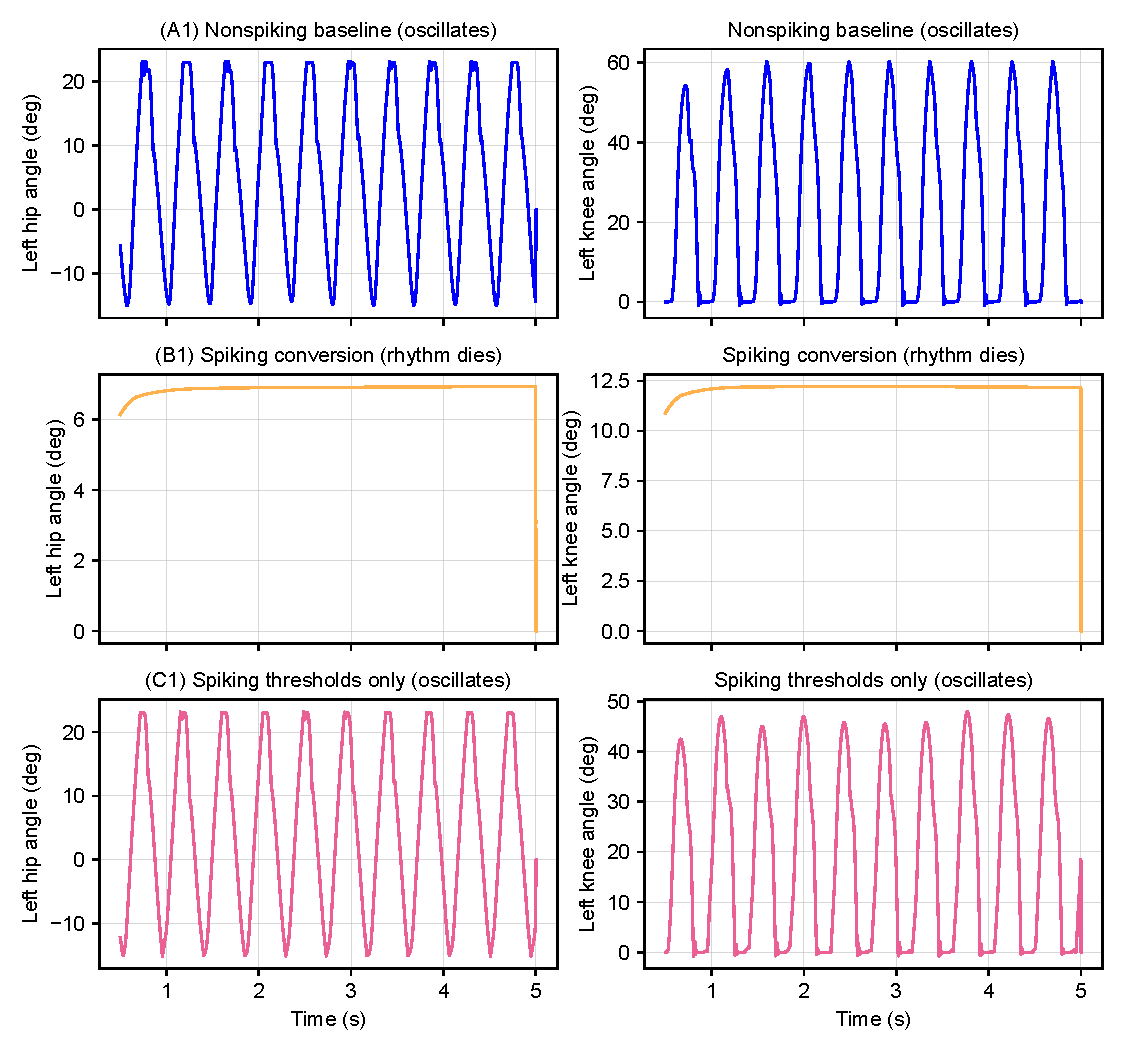
\includegraphics[width=\textwidth]{animatlab_spiking_conversion.pdf}
% ALT TEXT: see animatlab_spiking_conversion_alt.txt beside the figure file.
\caption{AnimatLab left hip (left column) and knee (right) angles over \qtyrange{0.5}{5}{\second}: \textbf{(A1)} nonspiking baseline, \textbf{(B1)} full spiking conversion, and \textbf{(C1)} spiking thresholds with voltage-dependent synapses retained.}
\label{fig:spike_animatlab}
\end{figure}

The converted AnimatLab models ran from their exported files. The nonspiking Simulink spinal model has 410 neurons and 1,392 synapses. Converting that model to spike-based signaling and fitting the separate MuJoCo network variants for spiking control were outside these comparisons.

\section{Connectome of the Verified W2L Model}\label{app:connectomes}
\graphicspath{{../Figures/93-AppendixB/}{figs/93-AppendixB/}}

The W2L walker used in Section~\ref{sec:app_supported_replays} has a bilateral controller that receives foot contact and limb-force signals. Its compiled network specifies which connections could transmit those signals between the two legs (Figures~\ref{fig:app_circuit_full} and~\ref{fig:app_circuit_core}). Built from the saved configuration \nolinkurl{w2l_verified_config.json}, this network has 96 neurons, 204 chemical synapses, and 22 input channels. The earlier spiking comparison used the separate 410-neuron Gait2392 controller.

The two sides each contain 48 neurons. RG and PF are the rhythm-generator and pattern-formation cells, and RG-IN and PF-IN are their local interneurons. MN denotes motor neurons, RC Renshaw cells, and Ia-IN reciprocal-inhibition interneurons. Ia, Ib, and II label muscle-afferent populations. In this controller, four heel and toe channels carry foot contact. Six Ib input channels on each side receive the same normalized extensor-force signal for that side. The other inputs are two initiation channels and four tonic-drive channels. The compiled input list contains no separate muscle-length or velocity channels for Ia or II. The c1 and V3 commissural interneurons follow the organization of \citet{shinohara_mechanisms_2025}. c1 inhibits the opposite flexor rhythm generator, and V3 excites contralateral extensor interneurons. Motor outputs drive six actuator channels per side.

Figure~\ref{fig:app_circuit_full} groups individual connections by their presynaptic and postsynaptic populations. A symbol indicates at least one connection of that sign; a population pair can contain both excitatory and inhibitory connections. The diagonal quadrants contain within-side pathways, and the other quadrants show interleg pathways. The matrix exposes the sensory projections to both RG and PF populations as well as to motor circuitry.

\begin{figure}[p]
\centering
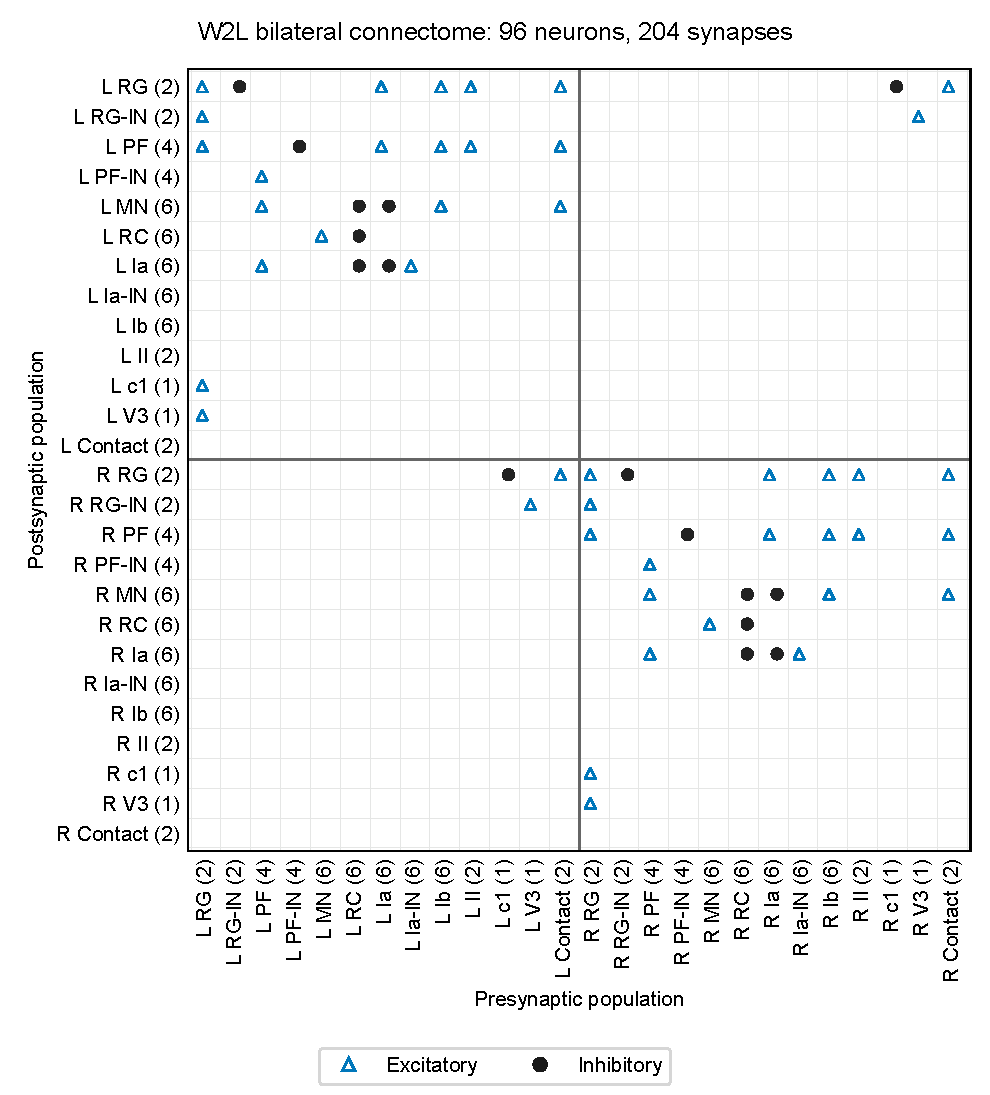
\includegraphics[width=\textwidth,height=0.82\textheight,keepaspectratio]{w2l_connectome_current.pdf}
\caption{Population connectivity of the verified W2L network. Parentheses give neuron counts. Open triangles denote excitation, and filled circles inhibition.}
\label{fig:app_circuit_full}
\end{figure}

Figure~\ref{fig:app_circuit_core} groups the maximum conductance of each synapse by its target population. Coincident points represent equal conductances. The spread shows how strengths differ within a pathway family. To determine what the contact and force pathways contribute during ground stepping, Appendix~\ref{sec:app_w2l_perturbations} compares the same walker in a virtual harness with selected connections enabled or removed.

\begin{figure}[htbp]
\centering
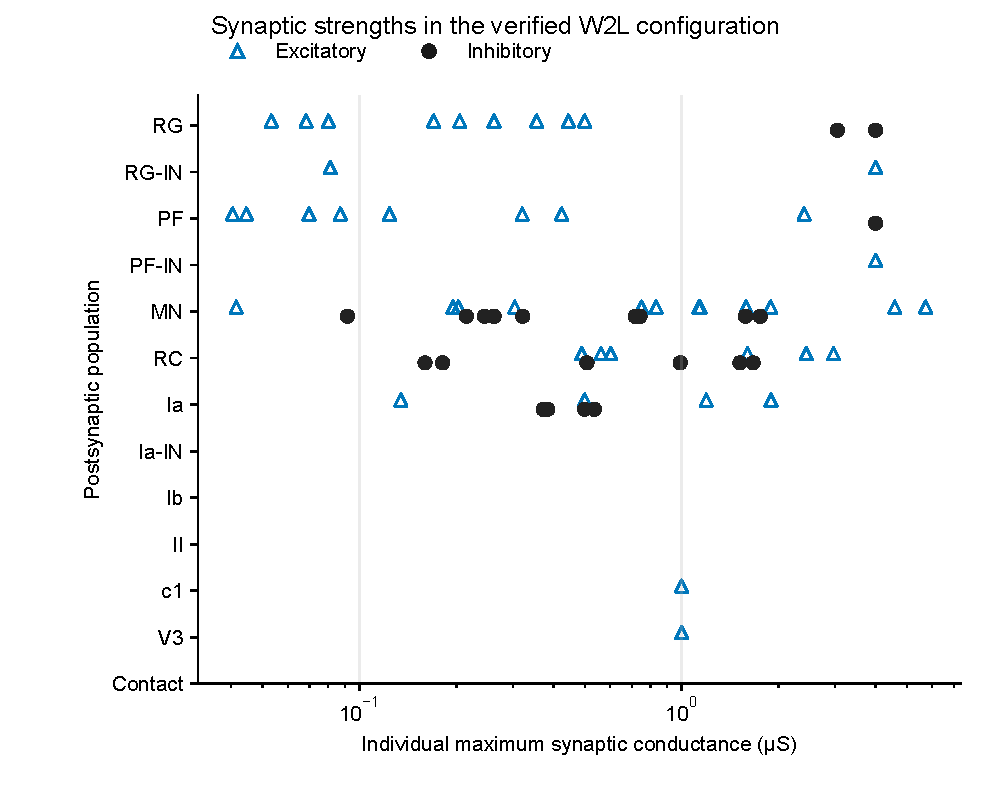
\includegraphics[width=\textwidth]{w2l_conductances_current.pdf}
\caption{Synaptic conductances in the verified W2L configuration, grouped by target population. The horizontal axis is logarithmic; coincident values overlap.}
\label{fig:app_circuit_core}
\end{figure}
